\section{Evaluation}
\label{sec:hyperscanner:eval}
We perform an initial experiment to evaluate the speedup in discovering classic Bluetooth devices of our new multi-channel scanning protocol and bandwidth extension, over a conventional smartphone scanner.
%
For our target we chose the HC-05, a popular commodity off-the-shelf Bluetooth module used in several applications in an urban area. 
%
In fact this module is so popular that we even criminals use it to build credit card skimmers
%
We took 8 HC-05 devices and put them in an RF isolation box, isolating them from WiFi and other wireless signals.
%
We connected a USRP x300 in the box to sense all the requests transmitted by our tools, and the responses sent by the HC-05 devices.
% 
The USRP constantly records the entire 80 MHz Bluetooth band to a computer, capturing every single packet that is sent by any device in the setup.
% 
We first put a smartphone with a Bluetooth scanning Android app (we used Bluetana from chapter) in the box to use as the scanning tool.
%
We run scanning app in constant scanning mode (with default scan time settings) to discover all the eight HC-05 devices.
%
We record all classic Bluetooth packets using the x300 for 41 seconds ($>40.96s$), and then process and decode the recorded requests and responses.
%
We then perform the same experiment using a PlutoSDR with our bandwidth extension hardware, and running our multi-channel scanning protocol using a simple onboard software.
%

\begin{figure}[h!]
    \centering
    \begin{subfigure}{0.48\textwidth}
        %\centering
        %\captionsetup{justification=centering}
        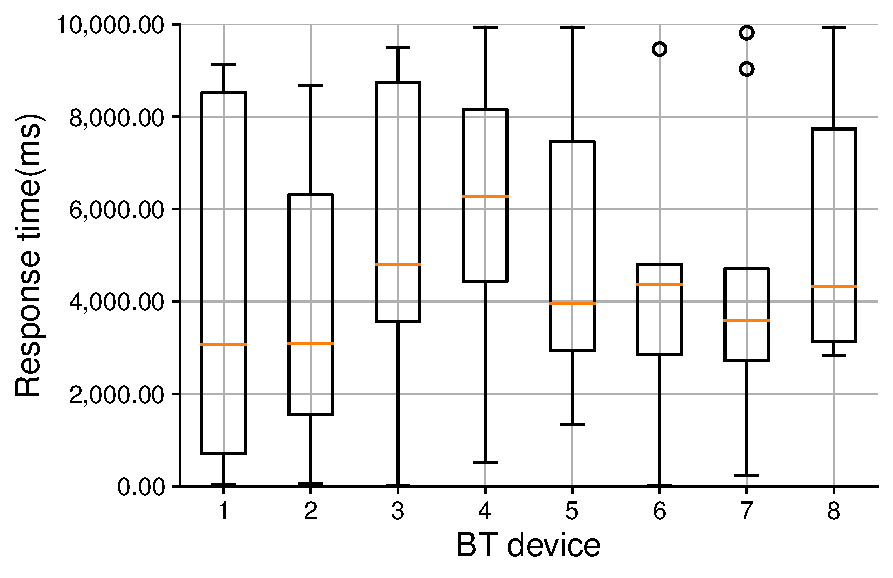
\includegraphics[width=\textwidth]{hyperscanner/plots/bluetana_default_out_inter_arrival_times.pdf}
        \caption{}
        %\label{fig:hyperscanner:bt_multi_chan}
    \end{subfigure}
    \hfill
    \begin{subfigure}{0.48\textwidth}
        %\centering
        %\captionsetup{justification=centering}
        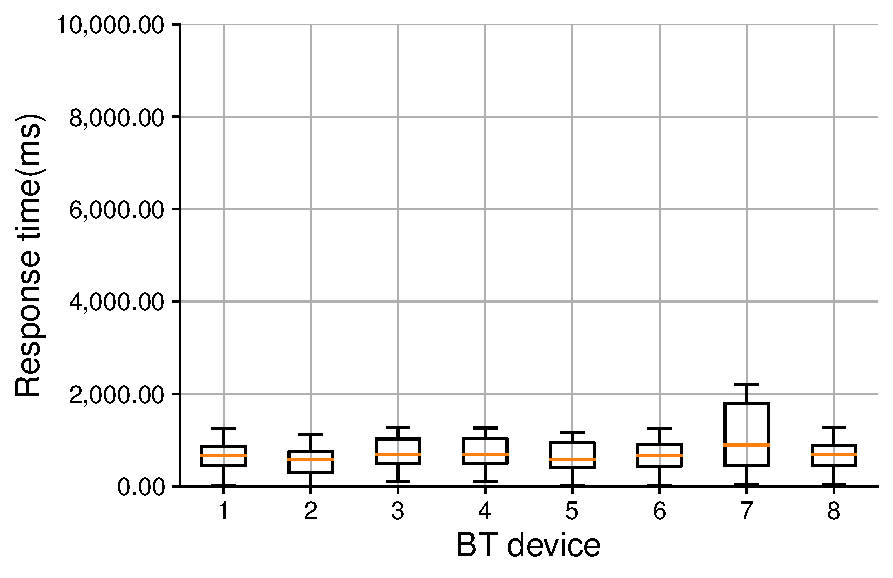
\includegraphics[width=\textwidth]{hyperscanner/plots/x300_26chan_switch_out_inter_arrival_times.pdf}
        \caption{}
        %\label{fig:hyperscanner:bt_multi_chan}
    \end{subfigure}
    \captionsetup{justification=centering}
    \caption{Empirical observations of Bluetooth device discovery time for (a) smartphone-based scanning tool (b) our improved low-cost scanning tool. Our tool significantly improves scan time, making it more effective for wardriving.}
    \label{fig:hyperscanner:fulltest}
\end{figure}

Figure~\ref{fig:hyperscanner:fulltest} shows the distribution of time to receive a response from each of the eight devices, across 10 tries of the experiment for both the smartphone scanner and our low-cost scanning tool.
%
We observe that the average time of discovery across the 8 devices improves from 4.88s to 0.71s for our low-cost scanner.
%
The variation in scan time from one trie to the next is significantly lower for our fast scanning tool.
%
Furthermore, we observe that the worst case scan time for any Bluetooth device goes down from 9.93s to 2.03s, making this tool extremely reliable and effective for wardriving data collection.

